\chapter{Introduction}

\section{White Dwarf Mergers}
\label{sec:wdmergers}

\subsection{The Panopoly of Stellar Mergers}
\label{ssec:stellarmergers}

Approximately two out of every three stars are born into a binary system.  A substantial fraction of these stars will interact, some due to their orbital separation at birth, while others following the expansion of one or both constituent stars as they evolve off of the main sequence.  These interactions primarily take form as mass transfer between the stars \citep{yung05}, and if mass transfer becomes unstable (increases exponentially over time), it ends with the violent coalescence of the two stars into one.  These stellar mergers, like other forms of binary interaction, disrupt single star evolution and create merged products, or ``merger remnants'', with unusual properties including blue stragglers (eg. \citealt{andrpt06, knigs09}), luminous blue variables \citep{justpv14}, subdwarf OB and R Coronae Borealis (RCrB) stars.

Mergers also liberate tremendous amounts of energy and eject significant amounts of mass, giving rise to a cornucopia of electromagnetic (and gravitational-wave) transients ranging from luminous red novae (from the merger of two (post-) main-sequence stars; eg. V838 Monocerotis and V1309 Scorpii \citep{tyle+11, nandil14}) to short gamma-ray bursts (from two neutron stars; eg. \citealt{ross15}) and the gravitational wave outburst from coalescing stellar-mass black holes (as recently found by the LIGO detector; \citealt{ligo16}).  Indeed, with current deep and short-cadence optical/near-infrared survey projects such as the Palomar Transient Factory \citep{rau+09} and Pan-STARRS \citep{kais+10} continuing to uncover more rare and even hitherto-unknown transients, and the ambitious Large Synoptic Survey Telescope \citep{lsst09} under construction, a much more complete picture of merger-generated transients will form over the next decade.

% Sec 5.2.3 of Tylenda talks about MS - MS pre-merger orbital evolution.

\subsection{Mergers of WD Binaries}
\label{ssec:c1_wdmergers_sub}

One common end-product of binary stellar evolution is a pair of white dwarf (WDs) in a close binary orbit.  These binaries are formed as a result of at least two phases of mass transfer (at least one of which is a common envelope event) during the binary's prior stellar evolution.  These mass transfer phases act to sap the orbital angular momentum of the 


SOMETHING SOMETHING YUNGELSON.

\subsubsection{WD Masses and Compositions}

\begin{figure}
\centerline{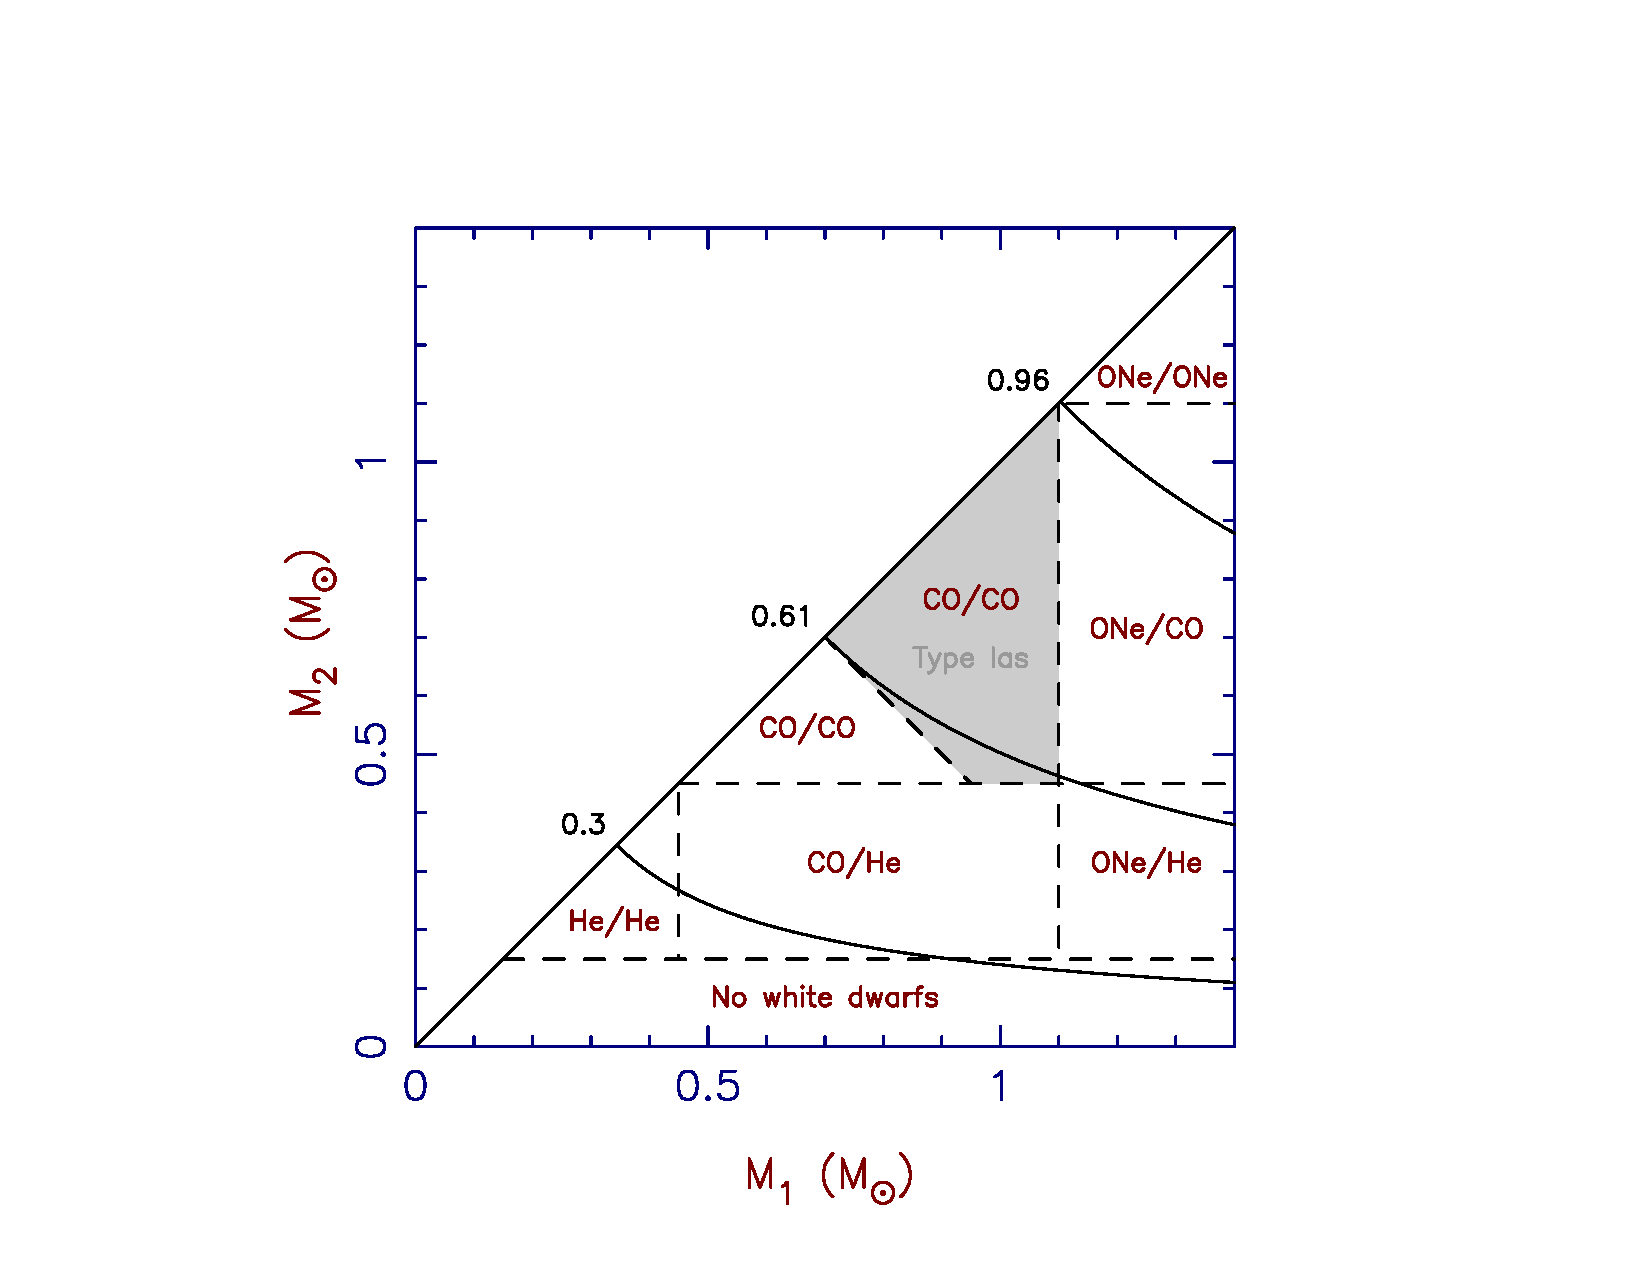
\includegraphics[width=0.6\hsize]{wdbinarymasses.pdf}
\caption{Plot of mass ratio ranges for WD binaries of various compositions.  Compositions were assumed to map uniquely onto mass via: He = $0.15 - 0.45\,\Msun$, CO = 0.45 - 1.1 {\Msun}, and ONe = 1.1 - 1.4 {\Msun}.  These values should be taken as guidelines, and not strict delinations between chemical compositions.  The curves are lines of constant gravitational wave chirp mass for inspiralling binaries.  The shaded region contains all CO WD binaries whose total mass is equal to or exceeds {\Mchan}, and are therefore expected to cause SNe Ia (see Sec. \ref{sec:withcarbon-oxygencompanions} for details.  From \cite{mars11}, their Fig. 1.}
\label{fig:c1_wdbinarymasses}
\end{figure}

WD mass and composition are both dependent on the evolutionary path of the WD progenitor star. A 0.15 - 0.45 {\Msun} WD will have a core comprised mostly of helium, a 0.45 - 1.1 {\Msun} WD will have a core of carbon and oxygen, and a 1.1 - 1.4 {\Msun} WD will have an oxygen-neon-magnesium core \citep{loreig09,mars11}.  (Work has been done, however, to show that these ranges are not set in stone; eg. \cite{moros09}.)  Brown dwarfs have masses of $\sim 0.08$ {\Msun} or lower \citep{stamw08}.

%A brown dwarf is a degenerate object composed largely of hydrogen, having never achieved the pressures and temperatures necessary for stable hydrogen burning.  While obviously formed from a very different stellar evolution channel, like WDs they are nonrelativistic degenerate bodies, and so obey the same stability arguments that have been detailed in the previous sections for white dwarfs.  Mergers between brown dwarfs, and between brown and white dwarfs, should be within the realm of physical possibility.

Close-in WD binaries are the result of common envelope evolution earlier in the binary's history.  Gravitational radiation or magnetic braking then drives the binary into a semi-detached state \citep{motl+07,nele+01}.  It is estimated that there are on order of $10^7$ - $10^8$ such semi-detached systems in the Milky Way alone \citep{motl+07,nele+01,mars11}.  Therefore any transients created by mass transfer within such systems should be frequently observed.

Statistically, mergers of certain types of WD binaries from Fig. \ref{wdbinarymasses} will dominate over others.  According to \cite{tremblay}, the mass distribution of DA white dwarfs (which comprise the vast majority of WDs) is narrowly peaked around $M = 0.65$ \Msun.  This suggests that the majority of WD binary interactions will be between near equal-mass CO WD pairs.  Binary evolution, however, will skew the population statistics of binary constituents.  \footnote{For example, in almost all cases a main-sequence binary system will undergo two stages of mass transfer to create a double degenerate system (one for the giant phase of each star).  The first phase of mass transfer must not result in common-envelope evolution; this requires a near-unity mass ratio between the two MS stars (see \cite{vkercj10} for details).  The most likely merger, then, is between two WDs of similar mass.}  \cite{han98} uses Monte Carlo simulations of binary evolution to determine that the birth rate of close-in WD binaries in the Milky Way is $\sim 3 \times 10^{-2}$ yr$^{-1}$, with 63\% being He-CO WD binaries, $\sim$ 2\% He-He, and 35\% CO-CO.  \citeauthor{han98} also gives merger rates: $5.7 \times 10^{-3}$ yr$^{-1}$ for He-He, $1.81 \times 10^{-2}$ yr$^{-1}$ for He-CO and $5.7 \times 10^{-3}$ yr$^{-1}$ for CO-CO mergers.  \cite{nele+01a}'s population sythesis models give different values for birth rates: a total rate of $4.8 \times 10^{-2}$ yr$^{-1}$, with 53\% of the binaries containing two He WDs, 25\% containing two CO WDs (including hybrid CO WDs with thick He envelopes), 20\% containing a CO and an He WD, and $\sim 1$\% containing ONeMg WDs.  The total merger rate for WDs of all sorts is $2.2 \times 10^{-2}$ yr$^{-1}$.  The differences between the two studies can be attributed to different common envelope inspiral efficiencies and treatments of mass transfer and stellar evolution.  (Each author also had multiple models with different treatments of such factors as star formation, WD cooling, etc.)

The frequency of BD-BD and BD-WD mergers has not been, to the best of our knowledge, quantified.


\subsubsection{Orbital Angular Momentum Loss and Gravitational Wave Emission}

Following their formation, these binaries can lose orbital angular momentum through a number of of mechanisms, including gravitational radiation (eg. \citealt{XXX}), magnetic braking \citep{XXX} or the influence of a third body \citep{XXX}.  {\charles TIDAL EFFECTS?  SOKER'S COMMON ENVELOPE MERGERS?}  In the absence of a magnetized wind or third body, gravitational radiation is generally thought to be the dominant driver of angular momentum loss, and has a characteristic timescale of \citep{segrcm97}

\eqbegin
\tau_{\mrm{grav}} = 5 \times 10^5 \left(\frac{a}{10^5 \mrm{km}}\right)^4 \frac{\Msun}{\Ma} \frac{\Msun}{\Md} \frac{\Msun}{\Mtot}\,\mrm{yr}.
\label{eq:c1_gravtimescale}
\eqend

\noindent From this, we see that WD binaries with orbital periods on the order of hours or less will merge within a Hubble time.  While inspiralling short-period WD binaries, with periods on the order of minutes, is too low-frequency to be detected by Advanced LIGO (Laser Interferometer Gravitational-Wave Observatory \citealt{ligo+15}), they are expected to be the most numerous and dominant source of gravitational waves \citep{mars11} detected by the proposed spaceborne detector eLISA (evolved Laser Interferometer Space Antenna; \citealt{amar+13}), which probes the mHz frequency range.  Signals from WD binaries in the years prior to merger can be individually resolved with eLISA at a few kpc \citep{loreig09, dan+11}, while the numerous sources further away will comprised an unresolved background \cite{neleyp01,amar+13}.  Note, however, that final coalescence of the WDs is over far too quickly to be detectable by eLISA.  The energy lost to gravitational radiation also plays a negligible role during the merger, being is $\sim10^{-10}$ of the binary's binding energy (eg. \citealt{loreig09}).

Like any merger, those between WDs liberate tremendous amounts of energy.  This can lead to enough heating and/or compression to reignite the nuclear furnaces of normally inert WDs under either non-degenerate or degenerate circumstances.  As such, the end product of such mergers are diverse, ranging from stars with unusual properties undergoing stable nuclear burning to explosions, the most powerful of which will resemble type Ia supernovae (SNe Ia), to be discussed shortly.  Which outcome occurs will largely depend on the compositions of the WDs involved, and we briefly summarize these below.

{\charles INSERT FIGURE OR CHART SUMMARIZING THE INFO BELOW?}

\subsubsection{Helium - Helium WD Mergers}



For two helium WDs, a low-mass helium star might result, which would be observed as an sdOB star.  

For a helium WD merging with a carbon-oxygen one, a helium giant could form, observable as a hydrogen-deficient giant or RCrB star.  

For two carbon-oxygen WDs (CO WDs), the outcome could vary between simply a more massive WD, a carbon-burning star, an explosion, or collapse to a neutron star, depending on whether stable or unstable carbon fusion is ignited, and whether the total mass exceeds the critical mass for pycnonuclear ignition or electron captures (both close to the Chandrasekhar mass \Mch).  For mergers involving an oxygen-neon WD, the mass will always be high, and explosive demise or transmutation seems inevitable.

White dwarf (WD) binaries are common end products of binary stellar evolution.  Gravitational wave emission, magnetic braking or the influence of a third body will cause a fraction of these to merge, producing a diversity of unusual stars and electromagnetic transients.  In particular, for double carbon-oxygen (CO) WD mergers, the final outcome could be a massive and rapidly rotating WD (eg. \citealt{segrcm97}), an accretion-induced collapse into a neutron star (NS) \citep{saion85}, or a nuclear explosion that might resemble a type Ia supernova (SN Ia).

%The merger of two white dwarfs (WDs) originally in a short-period binary is estimated (eg. \citealt{badem12}) to occur about once every century in a Milky Way-like galaxy, making the products of such events common throughout the universe.  They have been held responsible for producing a variety of stars with strange properties, including helium-burning sdOB stars \citep{saioj00, justph11}, RCrB stars (eg. \citealt{webb84, clay+07, clay13}), and massive and highly magnetized WDs (eg. \citealt{segrcm97, garc+12, kule+13}) that could resemble the hot DQ WDs (eg. \citealt{dunlc15}, Dunlap and Clements in preparation).  They may, however, also be responsible for spectacular transient events including accretion-induced collapses (eg. \citealt{saion85, abdi+10}) and type Ia supernovae (SNe Ia; eg. \citealt{howe11, hill+13, maozmn14}).  Determining the final outcome of a particular merger requires an understanding of the detailed dynamics of the merging process, which cannot directly be seen using current observational capabilities.  Thus, studies of merger physics have primarily utilized hydrodynamic simulations.
